
% this file is called up by thesis.tex
% content in this file will be fed into the main document

%: ----------------------- introduction file header -----------------------
\begin{savequote}[50mm]
Historical methodology, as I see it, is a product of common sense applied to circumstances. 
\qauthor{Samuel E. Morison}
\end{savequote}


\chapter{Método para la evaluación de competencias genéricas}
\label{cha:Overall methodology}

% the code below specifies where the figures are stored
\ifpdf
    \graphicspath{{4_overall_methodology/figures/PNG/}{4_overall_methodology/figures/PDF/}{4_overall_methodology/figures/}}
\else
    \graphicspath{{4_overall_methodology/figures/EPS/}{4_overall_methodology/figures/}}
\fi


%------------------------------------------------------------------------- 

En este capítulo se propone un método para la evaluación de competencias genéricas a partir de indicadores obtenidos del registro de interacciones de los estudiantes con el VLE. El capítulo comienza con una introducción a las bases de la propuesta y una descripción de las características más relevantes del \emph{learning analytics}. Finalmente se describirá la metología propuesta, las técnicas con las que se aplican y las implementaciones que se han realizado.

\section{Introducción}

Se podria decir que hoy en día el VLE es una pieza fundamental en cualquier contexto en el que se impartan cursos. Mientras que en los cursos virtuales es el único entorno de trabajo posible, en los cursos presenciales actúa como soporte virtual de las clases. Pero en ambos casos ofrece el espacio para gestionar el material del curso, las actividades y los estudiantes. 

Los estudiantes pasan a diario por las páginas del VLE. Por una lado, habrá estudiantes que entren en el sistema varias veces al día a consultar cualquier novedad y que sólo permanezcan 20 segundos en el VLE. Mientras que por otro lado, habrá estudiantes que entren una vez a la semana pero estén dos horas navegando por el VLE. Y entre un tipo de estudiante y otro, habrá tantas maneras de actuar de los estudiantes en el VLE como estudiantes haya. 

Todos los movimientos de los estudiantes quedan almacenados en el registro del VLE y estos registros podrían ser analizados para comprender el proceso de aprendizaje que en el VLE se está desarrollando. El \emph{learning analytics} es un area de investigación del aprendizaje mejorado por la tecnologia (TEL, del inglés \emph{Technology Enhanced Learning}) que esta enfocado en el desarrollo de métodos para analizar y detectar patrones en los datos recogidos en los entornos educativos y aprovecharlo para mejorar el aprendizaje~\cite{chatti2014learning}. La propuesta de esta tesis es que a partir de este método, los profesores podrán utilizar patrones de comportamiento de los estudiantes, plasmado a partir de su actividad en el VLE, como indicadores del desempeño de los estudiantes en las competencias genéricas. 

Este capítulo continua con los requisitos de método, la descripción detallada del mismo y su implementación en diferentes actividades de aprendizaje.

\section{Requisitos}

El método debe cumplir una serie de requisitos que parten de los inconvenientes encontrados en la revisión de la literatura realizada en el capítulo \ref{cha:State of the Art} y que han sido resumidos en el capítulo \ref{cha:Problemas}. A continuación se describe cada uno de estos requisitos.

\paragraph*{Indicadores objetivos}

Los indicadores reflejarán los datos obtenidos directamente del registro del VLE, por lo que serán objetivos per sé. No ha lugar a consideraciones personales o interpretaciones inexactas de rúbricas cómo ocurría en la autoevaluación o evaluación entre iguales, dónde dos evaluaciones de un mismo trabajo realizada por personas diferentes podria tener calificaciones diferentes. En el caso de los indicadores obtenidos del registro del VLE, dos estudiantes que tienen los mismos datos en el registro tendrán en el mismo valor en el indicador, y ya sera cometido del profesor la interpretación que otorgue a ese indicador.

\paragraph*{Evaluación escalable}

El método para la evaluación de competencias genéricas deberá ser escalable y no podrá suponer al profesor un esfuerzo que éste no pueda abordar. Por eso, el método se alineará con las herramientas del VLE, el profesor podrá consultar los indicadores del registro que requiera para llevar a cabo sus evaluaciones y la información será devuelta en formatos que el profesor pueda visionar y exportar a otras herramientas.

\paragraph*{Propósito general}

El próposito del método es obtener indicadores del registro del VLE y que estos sean utilizados para evaluar competencias genéricas. Pero no estan orientados a una competencia genérica concreta, sino que la idea es que el profesor diseñe sus actividades en el VLE y que luego obtenga los indicadores para utilizarlos en la evaluación de la competencia genéricas que considere que los estudiantes han desempeñado en dicha tarea (y que queda reflejada en los indicadores). El profesor podria incluso utilizar los indicadores para evaluar competencias específicas si lo creyese oportuno. Pero en ningún caso este método tendrá como propósito una competencia y actividad concreta como ocurría, por ejemplo, con algunos juegos serios recogidos en el estado del arte.

\paragraph*{Coste asumible}

No será necesario que el profesor tenga un perfil informático u otro específico para poder realizar las consultas de los indicadores. La interfaz en la que se implemente el método será lo más usable y sencilla posible para que los profesores puedan utilizarla sin requerirles conocimientos técnicos.

\paragraph*{Diseño de evaluaciones}

El método deberá proporcionar al profesor la posibilidad de diseñar sus propias evaluaciones a partir de los indicadores. En el estado del arte nos encontramos con trabajos que obtenían sus evaluaciones a partir de los indicadores del VLE, pero éstos eran fijos. Es decir, cada competencia se evalúa con un indicador dado. Pero puede ocurrir que el profesor no utilice las actividades del VLE que proporcionen dichos indicadores o que utilice las actividades con un enfoque diferente. También podría ocurrir que quisiera combinar el resultado de un indicador con otro para obtener lo que él considerará un indicador válido de la competencia. 

En resumen, podemos decir que el método que se propone para evaluar competencias genéricas a partir de los registros de interacción del VLE será puesto a disposición del profesor en forma de una herramienta informática que se conecte al VLE utilizado en la asignatura. Mediante esta herramienta, los profesores podran diseñar evaluaciones a partir de indicadores objetivos obtenidos del VLE y aplicarlas a las competencias genéricas para las que ellos consideren que les son válidos.


%\section{Learning analytics}

%Este término ya apareció en capítulos anteriores, pero es necesario volver a traerlo y hablar más en profundidad sobre él ya que es la base del método presentado en estre trabajo. El \emph{learning analytics} es la medición, recopilación, análisis y presentación de datos sobre los estudiantes, sus contextos y las interacciones que allí se generan, con el fin de comprender el proceso de aprendizaje que se está desarrollando y optimizar los entornos en los que se produce~\cite{siemens2012learning}.

\section{Descripción}

El método para la evaluación de competencias genéricas a partir de los registros del VLE se basa en el \emph{ciclo de contraste de hipótesis}. Este ciclo será explicado a continuación junto con el conjunto de pasos que explican el método.

\begin{enumerate}
\item Los estudiantes comienzan a dejar constancia de su actividad en el VLE desde el momento en que se registran en el sistema. El registro lo almacena todo, tanto la participación activa del estudiante, escribiendo y respndiendo mensajes en los foros o enviando actividades, como la participación pasiva, cuando simplemente lee el foro o se descarga los apuntes. 
\item Los programas de las asignaturas incluyen las competencias genéricas de las que los estudiantes deben ser evaluados. Los profesores pueden plantear actividades en el VLE con la intención no solo de evaluar ciertas habilidades de los estudiantes, sino también para provocar o conocer cómo lo resuelven los estudiantes. El fin de conocer el modo de proceder de los estudiantes es encontrar patrones de comportamiento que puedan ser interpretados como un indicador del desempeño de alguna competencia genérica.
\item Para evaluar una competencia genérica dada, el profesor podrá diseñar una evaluación a partir de la información contenida en el registro del VLE. Aquí comienza el  \emph{ciclo de contraste de hipótesis}. Ese diseño será procesado por el sistema que implementa el método y que terminará devolviendo la información al profesor. El resultado de aplicar el diseño será un indicador que el profesor podrá utilizar para la evaluación de la competencia genérica.
\item También se puede dar el caso de que el profesor considere que el indicador no es válido para la evaluación de la competencia genérica. También puede que aunque le sea válido pero considere que un rediseño del mismo le permitará afinar más en cuánto al ojetivo de evaluación de competencia genérica que se marcó. El profesor podría diseñar una nueva evaluación a partir de la información contenida en el registro y así sucesivamente hasta que los resultados satisfagan su hipótesis, momento en el que termina el  \emph{ciclo de contraste de hipótesis}.
\end{enumerate}

\section{Implementaciones}

Hay diversos entornos en los que se pueden desarrollar actividades de aprendizaje. Para la implementación del método se seleccionaron tres entornos diferentes: el primer entorno fue un wiki, entorno de trabajo online donde los usuarios crean y editan el contenido de forma colaborativa; el segundo fue un VLE, entorno de aprendizaje virtual donde se alojan cursos virtuales; y el tercero un mundo virtual, donde los estudiantes afrontan situaciones de la vida real en un entorno de simulación virtual.

En los próximos apartados se describirá cada una de las herramientas implementadas para abordar el diseño de evaluaciones para estas actividades de aprendizaje.

%------------------------------------------------
\subsection{Wikis: AssessMediaWiki}

El uso educacional de los wikis para las experiencias de trabajo colaborativo mediante el uso de la tecnología está en auge debido a las numerosas ventajas que aporta sobre los modelos tradicionales~~\cite{elgort2008wiki}. Algunas de las ventajas sobre los medios tradicionales, ya sean en formato impreso o en documentos digitales, es que estos no llevan un registro de ediciones, no permiten la colaboración distribuída y asincrona y no pueden ser monitorizados mientras son completados por el profesor.

Una de las características interesantes de los wikis es que no sólo almacenan la información de la versión final de cada documento, sino que también almacenan todas las versiones intermedias creadas como resultado de las contribuciones hechas por cada usuario~\cite{trentin2009using}. Para evaluar el trabajo final de un grupo de estudiantes en una página del wiki nos bastaría con leer la última versión de dicha página, como haciamos con los métodos tradicionales. Sin embargo, gracias a que los wikis mantienen un registro con las diferencias entre las ediciones consecutivas de las páginas, se podria utilizar dicha información como indicadores para la evaluación de diferentes competencias~\cite{ortega2011new}. Las páginas creadas de manera colaborativa podrían ser evaluadas considerando la contribución de cada autor y las dinámicas de grupo en la creación de la página en tiempo real. Por desgracia, realizar una evaluación detallada de cada contribución realizada en el wiki es imposible de abordar por la gran cantidad de trabajo que eso implica cuando el número de usuario en el wiki es elevado y participan activamente.

En este trabajo se propone una herramienta para realizar una evaluación escalable y cualitativa del trabajo realizado en el wiki. Para ello se creó \emph{AssessMediaWiki} (AMW), una aplicación web que proporciona procedimientos de autoevaluación, evaluación entre iguales y evaluación del profesor a partir de una rúbrica para evaluar a los estudiantes.

\subsubsection{Metodología para la evaluación del trabajo en el wiki}

AssessMediaWiki es una aplicación web de código abierto que, al conectarse a una instalación MediaWiki, proporciona procedimientos de autoevaluación, evaluación entre iguales y evaluación del profesor, a la vez que mantiene información sobre esas evaluaciones. Los supervisores pueden obtener informes que ayudan en la evaluación de los estudiantes.

AssessMediaWiki implementa dos roles de usuario distintos: supervisores y estudiantes. Los estudiantes pueden elegir entre distintas opciones: evaluar una revisión, comprobar sus propias aportaciones evaluadas y verificar las evaluaciones ya enviadas. Por otro lado, los supervisores tienen un mayor número de opciones, como definir la rubrica que los estudiantes deberán completar al realizar sus evaluaciones, modificar los parámetros de los programas o vigilar las evaluaciones que los alumnos vayan haciendo.

En la figura~\ref{fig:AmwDiagram} puede verse un diagrama de flujo de trabajo que muestra el proceso de evaluación realizado sobre una página del wiki en la que participan varios estudiantes y el profesor. Este flujo de trabajo tiene tres fases: una primera fase en la que los estudiantes realizan sus trabajos en las páginas del wiki, una segunda fase de evaluación y una tercera fase de revisión del profesor.

\begin{figure}
  \begin{center}
    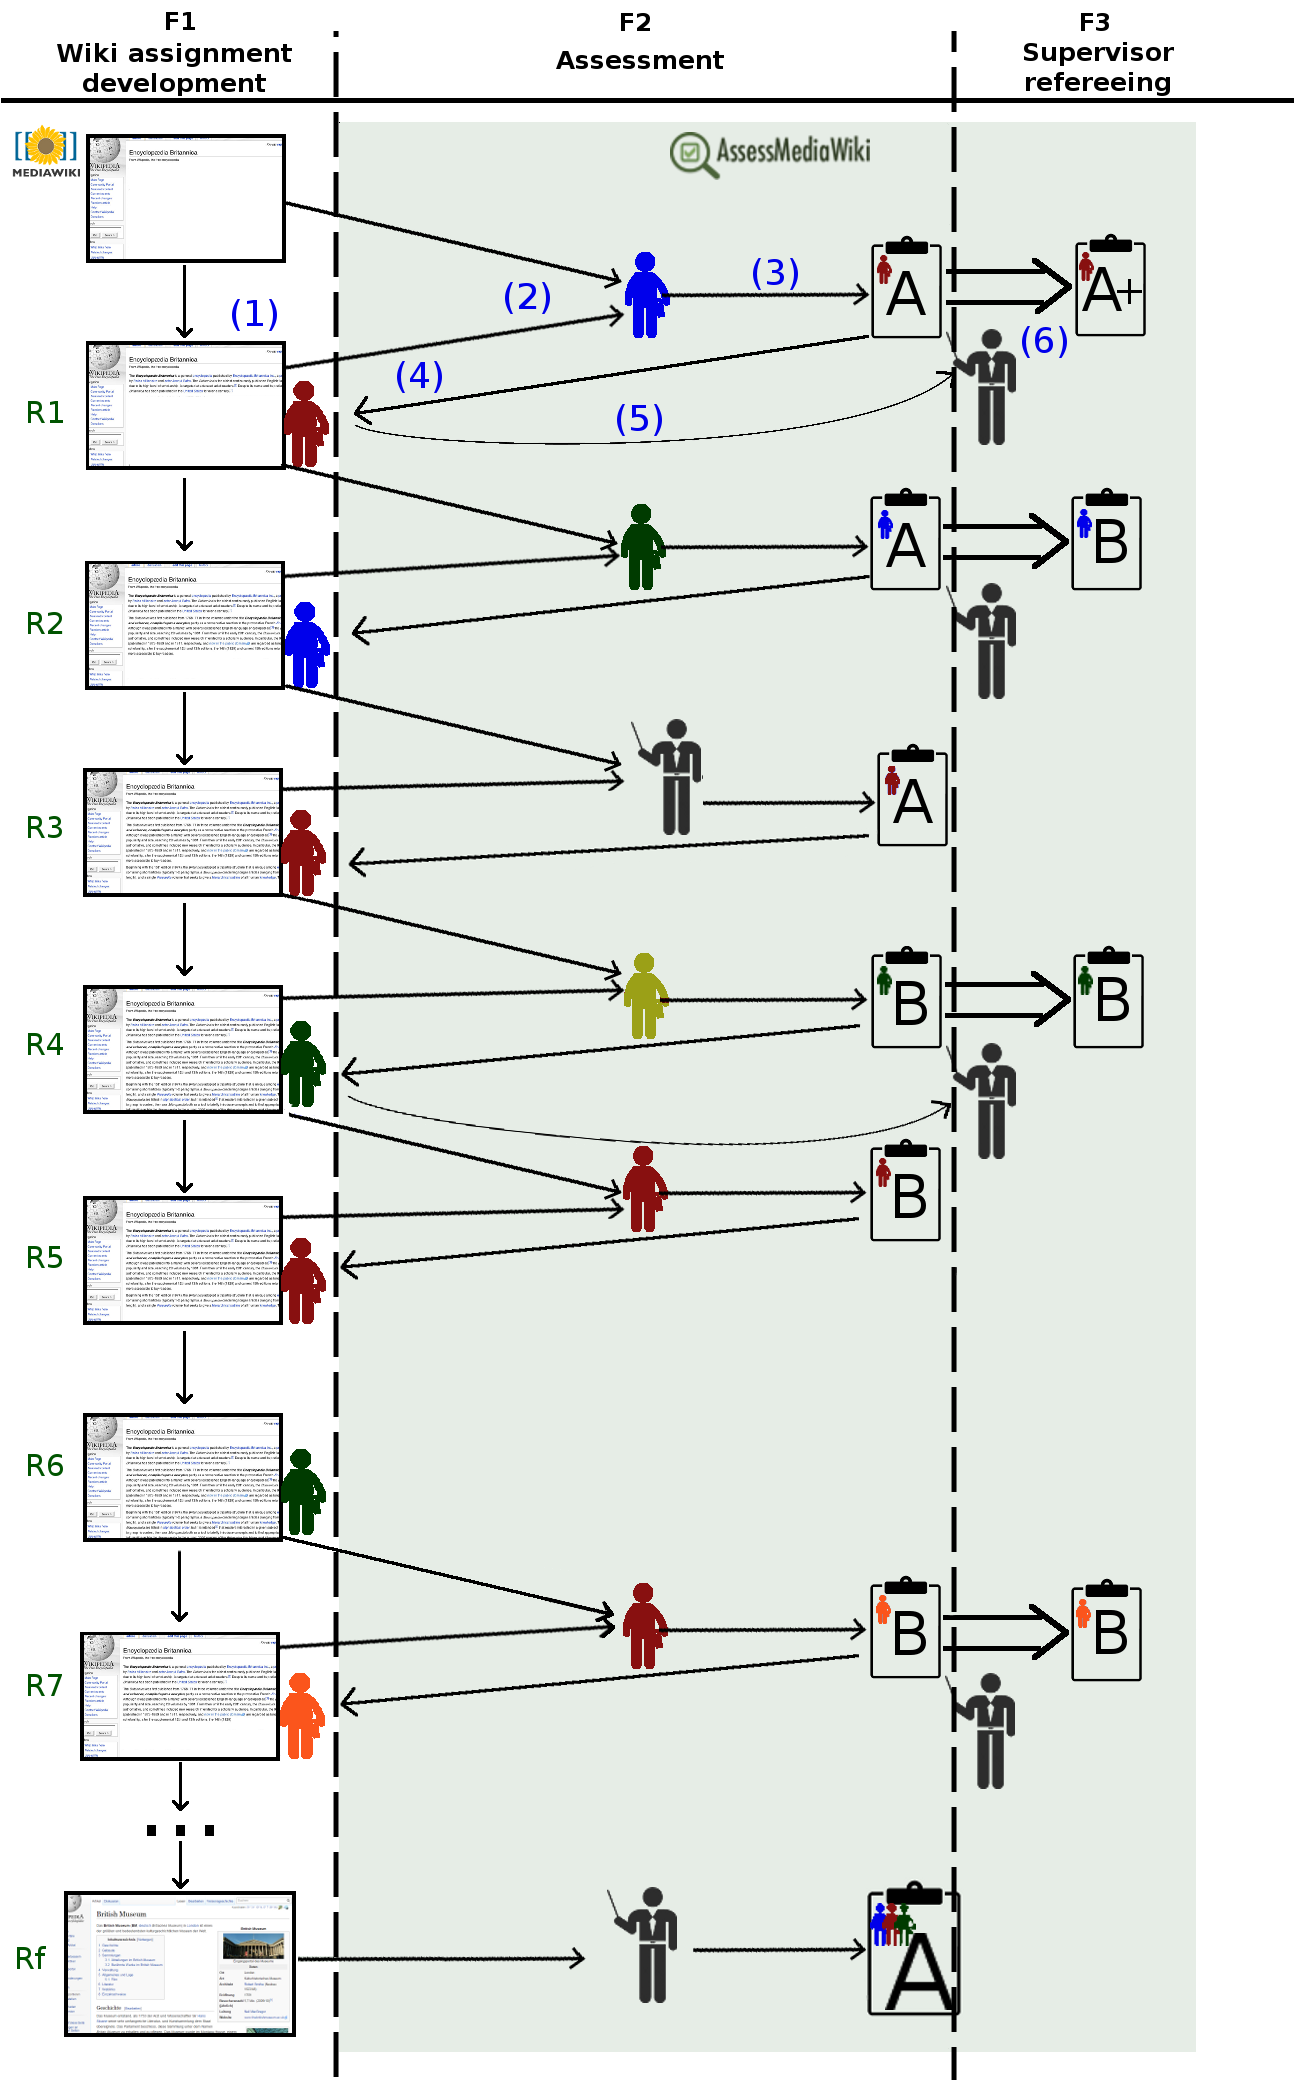
\includegraphics[scale=0.28]{AmwDiagram.png}
  \end{center}
  \caption{Ejemplo de flujo de trabajo para la evaluación cualitativa del wiki utilizando AMW}
  \label{fig:AmwDiagram}
\end{figure}

\paragraph*{Desarrollo del trabajo en el wiki}

Esta fase se representa en la columna de la izquierda de la figura~\ref{fig:AmwDiagram} y es en la que los estudiantes realizan el trabajo en las páginas del wiki. Normlamente, cada grupo de estudiantes tendrá que desarrollar su trabajos en una página del wiki. En la zona más alta de la columna se representa el comienzo del trabajo con una página en blanco. El autor de cada contribución se muestra con una figura de color junto a la misma. Para comenzar, el usuario de color rojo crea una página vacía (\emph{R1}). Después, el usuario azul añade contenido a la página (\emph{R2}). En tercer lugar, el usuario rojo modifica de nuevo la página añadiendo texto a la versión dejada anteriormente por el usuario azul (\emph{R3}) y así sucesivamente. Esta fase termina cuando llega la fecha marcada por el profesor para que los trabajos esten finalizados (\emph{Rf} es la versión final de la página).

Podemos también ver que aunque los estudiantes responsables de la página de ejemplo del wiki fuesen el rojo, el azul y el verde, otros estudiantes como en naranja en la revisión séptima podrían contribuir a la página del wiki. En ese caso, los miembros del grupo decidirían si la contribución debería conservarse o no.

\paragraph*{Evaluación}

Esta fase se muestra en la columna central y comprende las siguientes actividades:

\begin{itemize}
\item Autoevaluación, evaluación entre iguales y evaluación del profesor.
\item Revisión de las evaluaciones recibidas.
\item Réplica.
\item Evaluación final del wiki
\end{itemize}

\paragraph*{Revisión del profesor}

En esta última columna se representan dos actividades que corresponden al profesor:

\begin{itemize}
\item Resolución de las réplicas: el profesor revisa las réplicas indicando si proceden o no. En caso de que procedan, modifica la calificación. En el diagrama se puede ver como en en la primera contribución, el estudiante rojo realiza una réplica (\emph{5}) sobre la evaluación reciba por el usuario azul (\emph{3}). El profesor revisa la réplica, la considera apropiada y modifca la calificación (\emph{6}). En un segundo ejemplo, en la evaluación realizada por el estudiante de color amarillo sobre la contrbución realizada por el usuario de color verde puede verse como el profesor no acepta la réplica realizada por este último, y mantiene la calificación otorgada inicialmente por el estudiante amarillo.
\item Revisión de evaluaciones no replicadas: el profesor puede revisar aleatoriamente otras evaluaciones realizadas por los estudiantes que no hayan sido replicadas. En el diagrama puede verse como en el profesor revisa las evaluaciones realizadas sobre las contribuciones representadas en \emph{R2} y en \emph{R7}, disminuyendo la calificación de la primera y manteniendo la segunda.
\end{itemize}

\subsubsection{Herramienta}

bla bla bla

\subsubsection{Indicadores que aporta}

bla bla bla

\subsubsection{Ejemplo de uso}

bla bla bla

\subsubsection{Publicación}

bla bla bla
% La evaluación de las 3 herramientas se corresponde al capítulo siguiente.

%------------------------------------------------
\subsection{EvalCourse}

bla bla bla

\subsubsection{Descripción}

bla bla bla

\subsubsection{Tecnología implementada}

bla bla bla

\subsubsection{Indicadores que aporta}

bla bla bla

\subsubsection{Ejemplo de uso}

bla bla bla

\subsubsection{Publicación}

bla bla bla
% La evaluación de las 3 herramientas se corresponde al capítulo siguiente.

%------------------------------------------------
\subsection{EvalSim}

bla bla bla

\subsubsection{Descripción}

bla bla bla

\subsubsection{Tecnología implementada}

bla bla bla

\subsubsection{Indicadores que aporta}

bla bla bla

\subsubsection{Ejemplo de uso}

bla bla bla

\subsubsection{Publicación}

bla bla bla
% La evaluación de las 3 herramientas se corresponde al capítulo siguiente.


%Metolodogía mixta

%Cómo voy a evaluar roles, momentos, actividad, ... lo que sea.

%Explicar el DSL

%DSL: herramienta de investigación en evaluaciones. Esta herramienta ayuda al investigador a formalizar la evaluación.
 
%Enfocar la metodología a que no es una metodología para evaluar, sino para diseñar evaluaciones. Diseñador de evaluaciones.

%Explicar qué pasos tiene que seguir un diseñador de evaluaciones para hacer sus evaluaciones.

%Dentro de los resultados obtenemos dos cosas:
%1. Diseño
%2. Lo que el diseñador nos indicó que no pudo hacer

%Para que esto sea posible falta la herramienta informática

%\section{Evolución herramientas}

%AMW --> EvalCourse --> EvalSim

%\section{Metodologia de desarrollo}

%DSL? Ing. Dirigida x modelo?



% ----------------------------------------------------------------------

